\section{Theorie}
\label{sec:theorie}

\subsection*{Brechung}

Trifft Licht, also elektromagnetische Strahlung, auf eine Grenzfläche zwischen zwei verschiedenen Medien, wird der Lichtstrahl gebrochen, 
der Winkel, unter dem das Licht auf eine waagerechte Ebene treffen würden, ändert sich.

\begin{figure}[H]
    \centering
    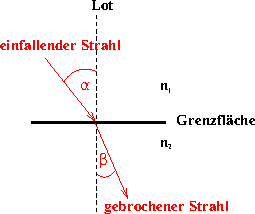
\includegraphics{figures/Abb_2b.pdf}
    \caption{Brechung eines Lichtstrahls an einem Grenzübergang zwischen Medium 1 und Medium 2 \cite{ap02}.}
    \label{fig:abb2b}
\end{figure}

Mit, wie in \autoref{fig:abb2b} dargestellt, verschiedenen Lichtgeschwindigkeiten $c_1$ und $c_2$ in den unterschiedlichen Medien gilt die Beziehung
\begin{equation}
    \frac{\sin(\alpha)}{\sin(\beta)} = \frac{c_1}{c_2} = \frac{n_2}{n_1} \,,
    \label{eq:brechungsgesetz}
\end{equation}
bzw.
\begin{equation}
    n_1 \sin(\alpha) = n_2 \sin(\beta) \,,
    \label{eq:snellius}
\end{equation}
wobei $n_i$ den Brechungsindex des $i$-ten Mediums darstellt. \\

Während das eine Medium im Regelfall Luft darstellt, können je nach Eigenschaften des anderen Stoffes verschiedene Fälle unterschieden werden. \\

\subsection*{Reflexion}

Wird ein Lichtstrahl an einer Oberfläche reflektiert, so ist der Einfallswinkel $\alpha_1$, \autoref{fig:abb2a} entsprechend, gleich dem Ausfallswinkel $\alpha_2$, also
\begin{equation}
    \alpha_1 = \alpha_2 \,.
    \label{eq:reflexion}
\end{equation} \\

\begin{figure}
    \centering
    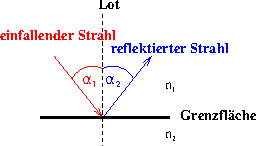
\includegraphics{figures/Abb_2a.pdf}
    \caption{Reflexion eines Lichtstrahl an einer Oberfläche \cite{ap02}.}
    \label{fig:abb2a}
\end{figure}

\subsection*{Reflexion und Transmission}

Normalerweise finden Reflexion und Brechung nicht einzeln, sondern gleichzeitig statt. Wie in \autoref{fig:abb2c} dargestellt wird ein Teil des Lichts mit der Intensität $I_r$ wird reflektiert, 
während der andere Teil des Lichts mit der Intensität $I_t$ transmittiert wird.

\begin{figure}
    \centering
    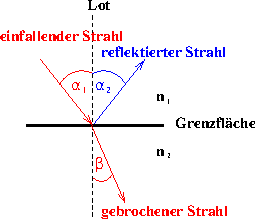
\includegraphics{figures/Abb_2c.pdf}
    \caption{Reflexion und Transmission an einer Grenzfläche zum Medium 2 \cite{ap02}.}
    \label{fig:abb2c}
\end{figure}

Dabei gilt stets
\begin{equation*}
    I_r + I_t = 1 \,,
\end{equation*}
auch wenn sich die Anteile reflektierter bzw. transmittierter Strahlung von Stoff zu Stoff unterscheiden können. \\

\subsection*{Beugung}

Bei der Beobachtung von Licht, das auf ein Hindernis trifft, lässt sich häufig feststellen, dass sich das Licht auch im Schattenraum hinter dem Hindernis ausbreitet.
Dieses Phänomen wird Beugung genannt und kann nicht mehr allein mithilfe der Strahlenoptik betrachtet werden.
Durch die Überlagerung zweier oder mehr Wellen entsteht ein Interferenzmuster, dessen Intensitätsverteilung von der Phasendifferenz der interferierenden Wellen entspricht.
Je nach Gangunterschied interferieren die Wellen konstruktiv oder destruktiv, verstärken sich also bzw. schwächen sich gegenseitig ab. \\

Nach dem Huygenschen Prinzip stellt ein Hindernis lediglich einen einfachen Spalt dar. 
Eine Welle der Frequenz $\nu$, Wellenlänge $\lambda$ und der Ausbreitungsgeschwindigkeit $v$, das im Winkel $\alpha$ durch einen Spalt der Breite $a$ auf einen Schirm im Abstand $L$ trifft, erzeugt ein Interferenzmuster
aus hellen und dunklen Streifen.

Diese hellen Streifen erscheinen an den Stellen, an denen mit $k \in \mathbb{N}$
\begin{equation}
    a \sin(\alpha) = k \lambda
    \label{eq:beugmaxeinzspalt}
\end{equation}
gilt. \\

Alternativ gilt für ein Strichgitter bestehend aus $N$ Einfachspalten gleicher Breite
\begin{equation}
    d \sin(\alpha) = k \lambda \,,
    \label{eq:beugmaxgitter}
\end{equation}
wobei $d$ die Gitterkonstante beschreibt.



